\section*{Návrh sítě}
\label{sec:network_design}

Pro popis jednotlivých stavů a přechodu na \figref{fig:network} bude využita zkratka $p_i$ pro místa a $t_i$ pro přechody, kde $i$ je identifikátor před dvojtečkou.

\begin{figure}[h!]
    \centering
    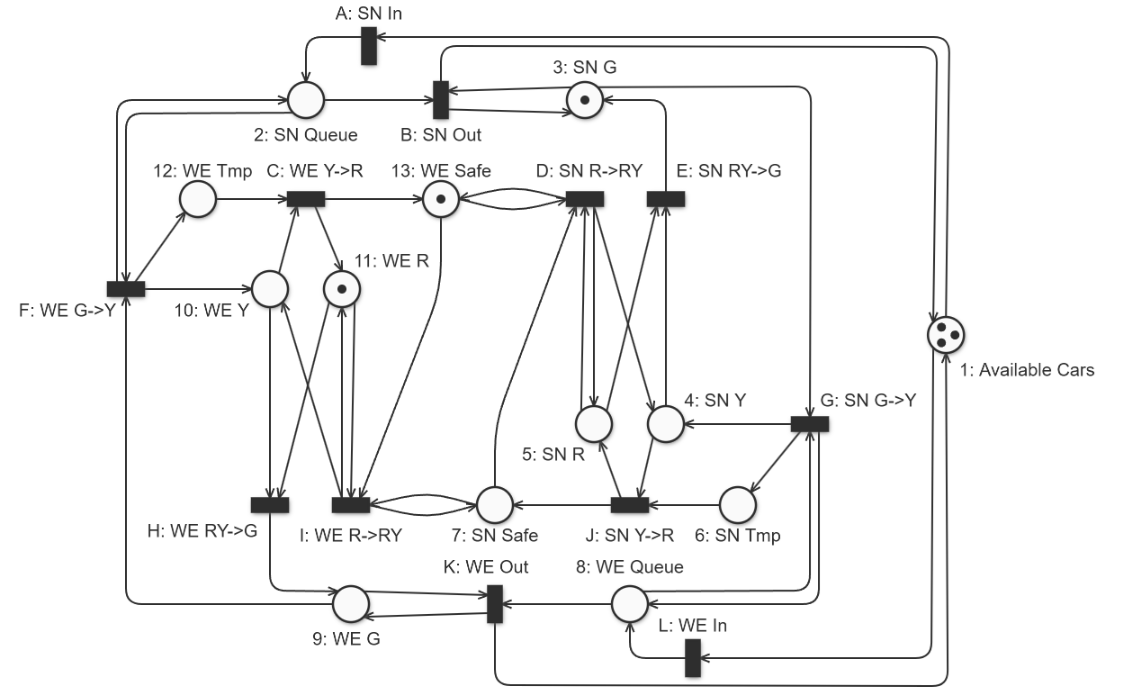
\includegraphics[width=0.85\textwidth]{assets/pes_network}
    \caption{Petriho síť reprezentující chování semaforů na křižovatce.}
    \label{fig:network}
\end{figure}

\begin{table}[h!]
    \centering
    \resizebox{0.50\textwidth}{!}{
        \begin{tabular}{c|c|c|c|c|c|c|c|c|c|c|c|c|}
            \textbf{} & \textbf{$t_a$} & \textbf{$t_b$} & \textbf{$t_c$} & \textbf{$t_d$} & \textbf{$t_e$} & \textbf{$t_f$} & \textbf{$t_g$} & \textbf{$t_h$} & \textbf{$t_i$} & \textbf{$t_j$} & \textbf{$t_k$} & \textbf{$t_l$} \\
            \hline
            %                  A      B      C      D      E      F      G      H      I      J      K      L
            \textbf{$p_1$}   & $-1$ & $+1$ & $  $ & $  $ & $  $ & $  $ & $  $ & $  $ & $  $ & $  $ & $+1$ & $-1$ \\
            \textbf{$p_2$}   & $+1$ & $-1$ & $  $ & $  $ & $  $ & $ 0$ & $  $ & $  $ & $  $ & $  $ & $  $ & $  $ \\
            \textbf{$p_3$}   & $  $ & $ 0$ & $  $ & $  $ & $+1$ & $  $ & $-1$ & $  $ & $  $ & $  $ & $  $ & $  $ \\
            \textbf{$p_4$}   & $  $ & $  $ & $  $ & $+1$ & $-1$ & $  $ & $+1$ & $  $ & $  $ & $-1$ & $  $ & $  $ \\
            \textbf{$p_5$}   & $  $ & $  $ & $  $ & $ 0$ & $-1$ & $  $ & $  $ & $  $ & $  $ & $+1$ & $  $ & $  $ \\
            \textbf{$p_6$}   & $  $ & $  $ & $  $ & $  $ & $  $ & $  $ & $+1$ & $  $ & $  $ & $-1$ & $  $ & $  $ \\
            \textbf{$p_7$}   & $  $ & $  $ & $  $ & $-1$ & $  $ & $  $ & $  $ & $  $ & $ 0$ & $+1$ & $  $ & $  $ \\
            \textbf{$p_8$}   & $  $ & $  $ & $  $ & $  $ & $  $ & $  $ & $ 0$ & $  $ & $  $ & $  $ & $-1$ & $+1$ \\
            \textbf{$p_9$}   & $  $ & $  $ & $  $ & $  $ & $  $ & $-1$ & $  $ & $+1$ & $  $ & $  $ & $ 0$ & $  $ \\
            \textbf{$p_1_0$} & $  $ & $  $ & $-1$ & $  $ & $  $ & $+1$ & $  $ & $-1$ & $+1$ & $  $ & $  $ & $  $ \\
            \textbf{$p_1_1$} & $  $ & $  $ & $+1$ & $  $ & $  $ & $  $ & $  $ & $-1$ & $ 0$ & $  $ & $  $ & $  $ \\
            \textbf{$p_1_2$} & $  $ & $  $ & $-1$ & $  $ & $  $ & $+1$ & $  $ & $  $ & $  $ & $  $ & $  $ & $  $ \\
            \textbf{$p_1_3$} & $  $ & $  $ & $+1$ & $ 0$ & $  $ & $  $ & $  $ & $  $ & $-1$ & $  $ & $  $ & $  $ \\
        \end{tabular}
    }
    \caption{Matice incidence Petriho sítě. \footnotemark}
    \label{tab:transitions}
\end{table}

\footnotetext[1]{Hodnoty 0 představují obousměrnou výměnu tokenu mezi místem. Hodnoty +1 a -1 značí přidání nebo odebrání tokenu z místa.}

\endinput